% The plane d1+d2+d3=6, projected onto orthonormal plane coordinates.
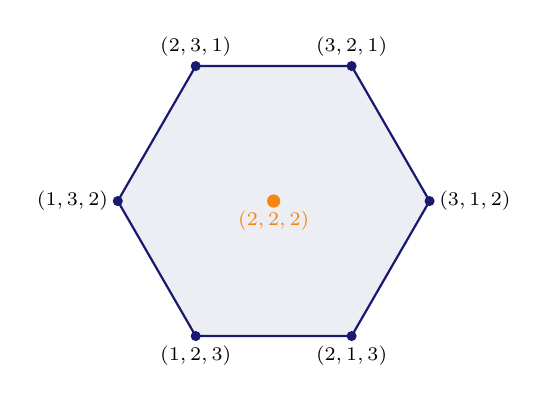
\begin{tikzpicture}[scale=1.4,every node/.style={font=\scriptsize}]
\fill[MidnightBlue!8] (0.7071,1.2247)--(1.4142,0)--(0.7071,-1.2247)--(-0.7071,-1.2247)--(-1.4142,0)--(-0.7071,1.2247)--cycle;
\draw[MidnightBlue,thick] (0.7071,1.2247)--(1.4142,0)--(0.7071,-1.2247)--(-0.7071,-1.2247)--(-1.4142,0)--(-0.7071,1.2247)--cycle;
\foreach \x/\y/\lab/\pos in {0.7071/1.2247/{(3,2,1)}/above,1.4142/0/{(3,1,2)}/right,0.7071/-1.2247/{(2,1,3)}/below,-0.7071/-1.2247/{(1,2,3)}/below,-1.4142/0/{(1,3,2)}/left,-0.7071/1.2247/{(2,3,1)}/above}{
\fill[MidnightBlue] (\x,\y) circle (1.3pt);
\node[\pos] at (\x,\y) {$\lab$};}
\fill[BurntOrange] (0,0) circle (1.7pt);
\node[BurntOrange,below] at (0,0) {$(2,2,2)$};
\end{tikzpicture}
